\documentclass[10pt]{beamer}

\usetheme[progressbar=frametitle]{metropolis}
\usepackage{appendixnumberbeamer}
\usepackage{amsmath}
\usepackage{amssymb}
\usepackage[russian]{babel}

\usepackage{booktabs}
\usepackage[scale=2]{ccicons}

\usepackage{pgfplots}
\usepgfplotslibrary{dateplot}

\usepackage{xspace}
\newcommand{\themename}{\textbf{\textsc{metropolis}}\xspace}

\usepackage{bm}
\usepackage{esint}

\newcommand{\pd}{\partial}
\newcommand{\br}{\bm{r}}
\newcommand{\bv}{\bm{v}}
\newcommand{\bu}{\bm{u}}
\newcommand{\bw}{\bm{w}}
\newcommand{\bc}{\bm{c}}
\newcommand{\bq}{\bm{q}}
\newcommand{\eps}{\varepsilon}
\newcommand{\be}{\bm{e}}
\newcommand{\bg}{\bm{g}}
\newcommand{\ab}{\alpha\beta}
\newcommand{\bn}{\bm{n}}
\newcommand{\kp}{\kappa}


\title{Компьютерное моделирование кинетического и
гидродинамического приближения сложных статистических систем}
\subtitle{Отчет о выполненных работах}
% \date{\today}
\date{}
\author{Ернур Байболатов}
\institute{STEM парк, КазНПУ им. Абая}
% \titlegraphic{\hfill\includegraphics[height=1.5cm]{logo.pdf}}

\begin{document}

\maketitle

\begin{frame}{Содержание}
  \setbeamertemplate{section in toc}[sections numbered]
  \tableofcontents[hideallsubsections]
\end{frame}

\section{Введение}

\begin{frame}[fragile]{Гранулярные газы}

  Гранулярными называются вещества состоящие из отдельных макроскопических тел

  \begin{figure}[h]
    \centering
    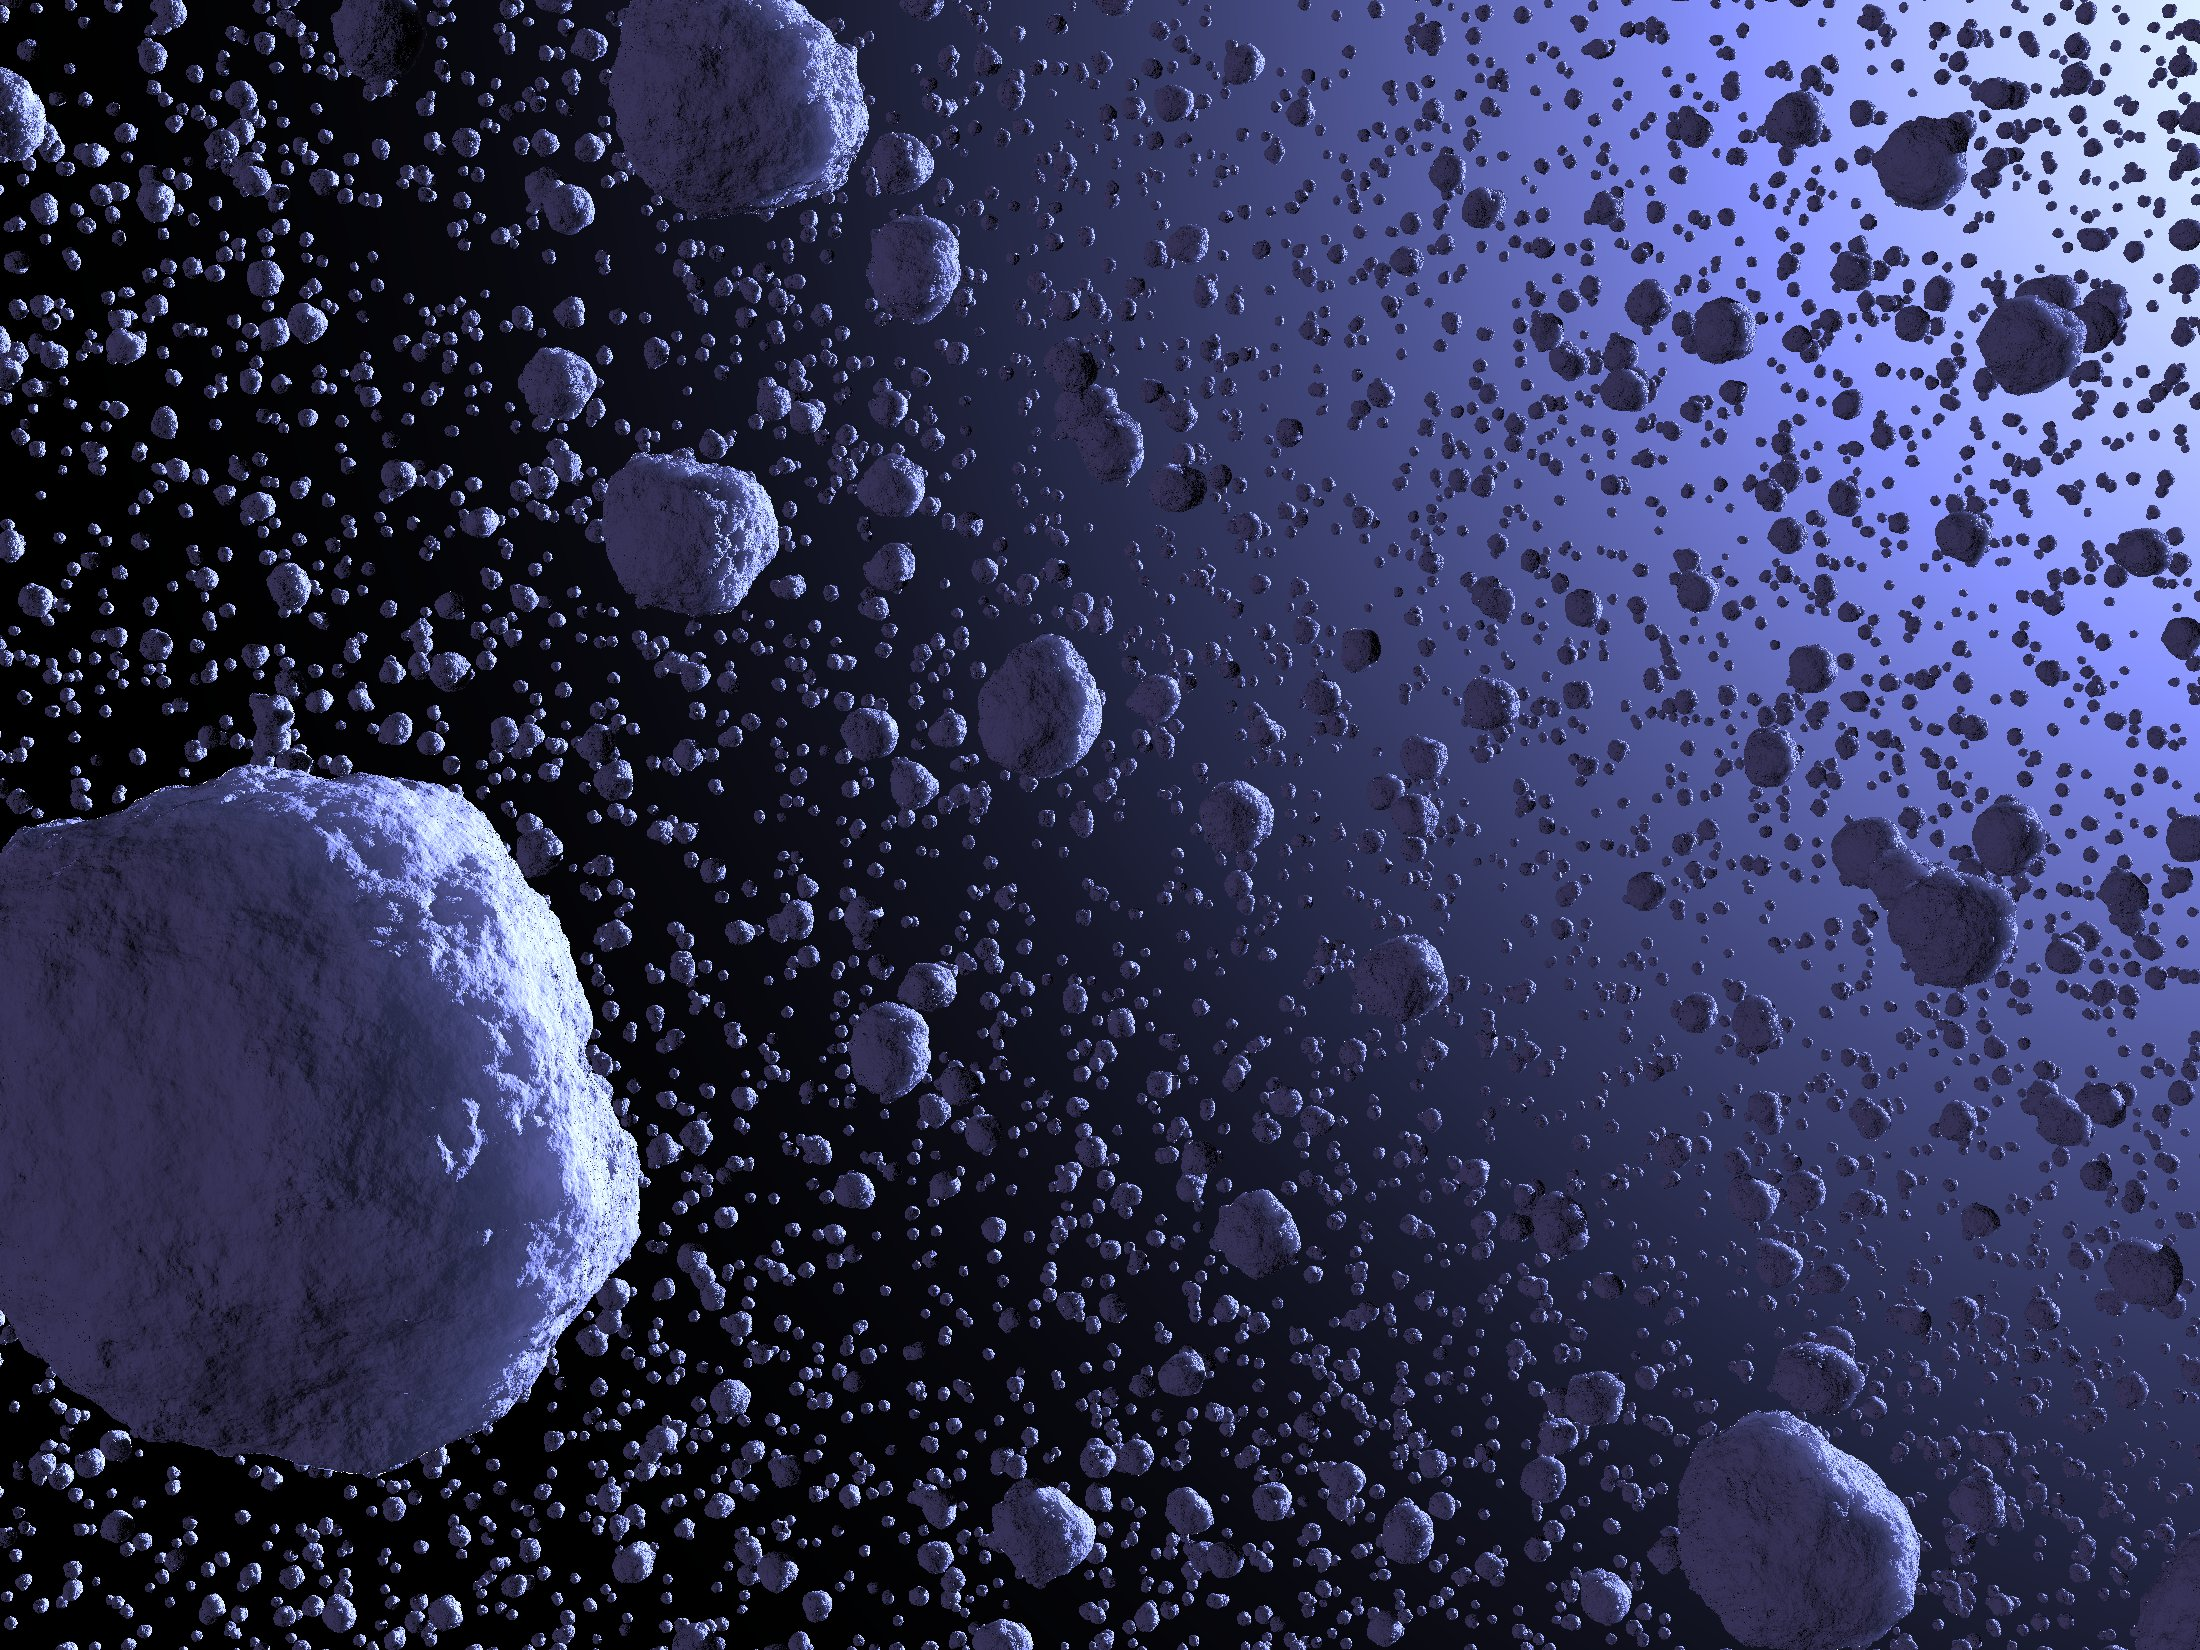
\includegraphics[width=0.77\textwidth]{gran_gas.jpg}    
    \label{fig:granular_gas}
  \end{figure}

\end{frame}

\begin{frame}[fragile]{Особенности}
  Основное свойство --- диссипативность. При каждом столкновении частиц, энергия системы понижается

  Коэффициент реституции
  \begin{equation}
    \bg'_{12} = -\varepsilon\bg_{12}
  \end{equation}
  где $0\leq\varepsilon\leq 1$.  
  
\end{frame}

\begin{frame}[fragile]{Гранулярная температура}
  По аналогии с термодинамической температурой

  \begin{equation}
    \frac{3}{2}T = \frac{1}{N}\sum_{i=1}^{N}\frac{m\bv_i^2}{2}
  \end{equation}
  
\end{frame}

\begin{frame}[fragile]{Закон Хаффа}
  По причине постоянной диссипации, предоставленный самому себе гранулярный газ
  постепенно охлаждается

  \begin{equation}
    T(t)=\frac{T_0}{\left(1+t/\tau_0\right)^2}\;,
  \end{equation}
  где 
  \begin{equation}
    \tau_0^{-1}\propto n\sigma^2\left(1-\varepsilon^2\right)\sqrt{T_0}
  \end{equation}
\end{frame}

\begin{frame}[fragile]{Кольца Сатурна}
  Природным примером массивных гранулярных газов являются планетарные кольца 

  \begin{figure}[h]
    \centering
    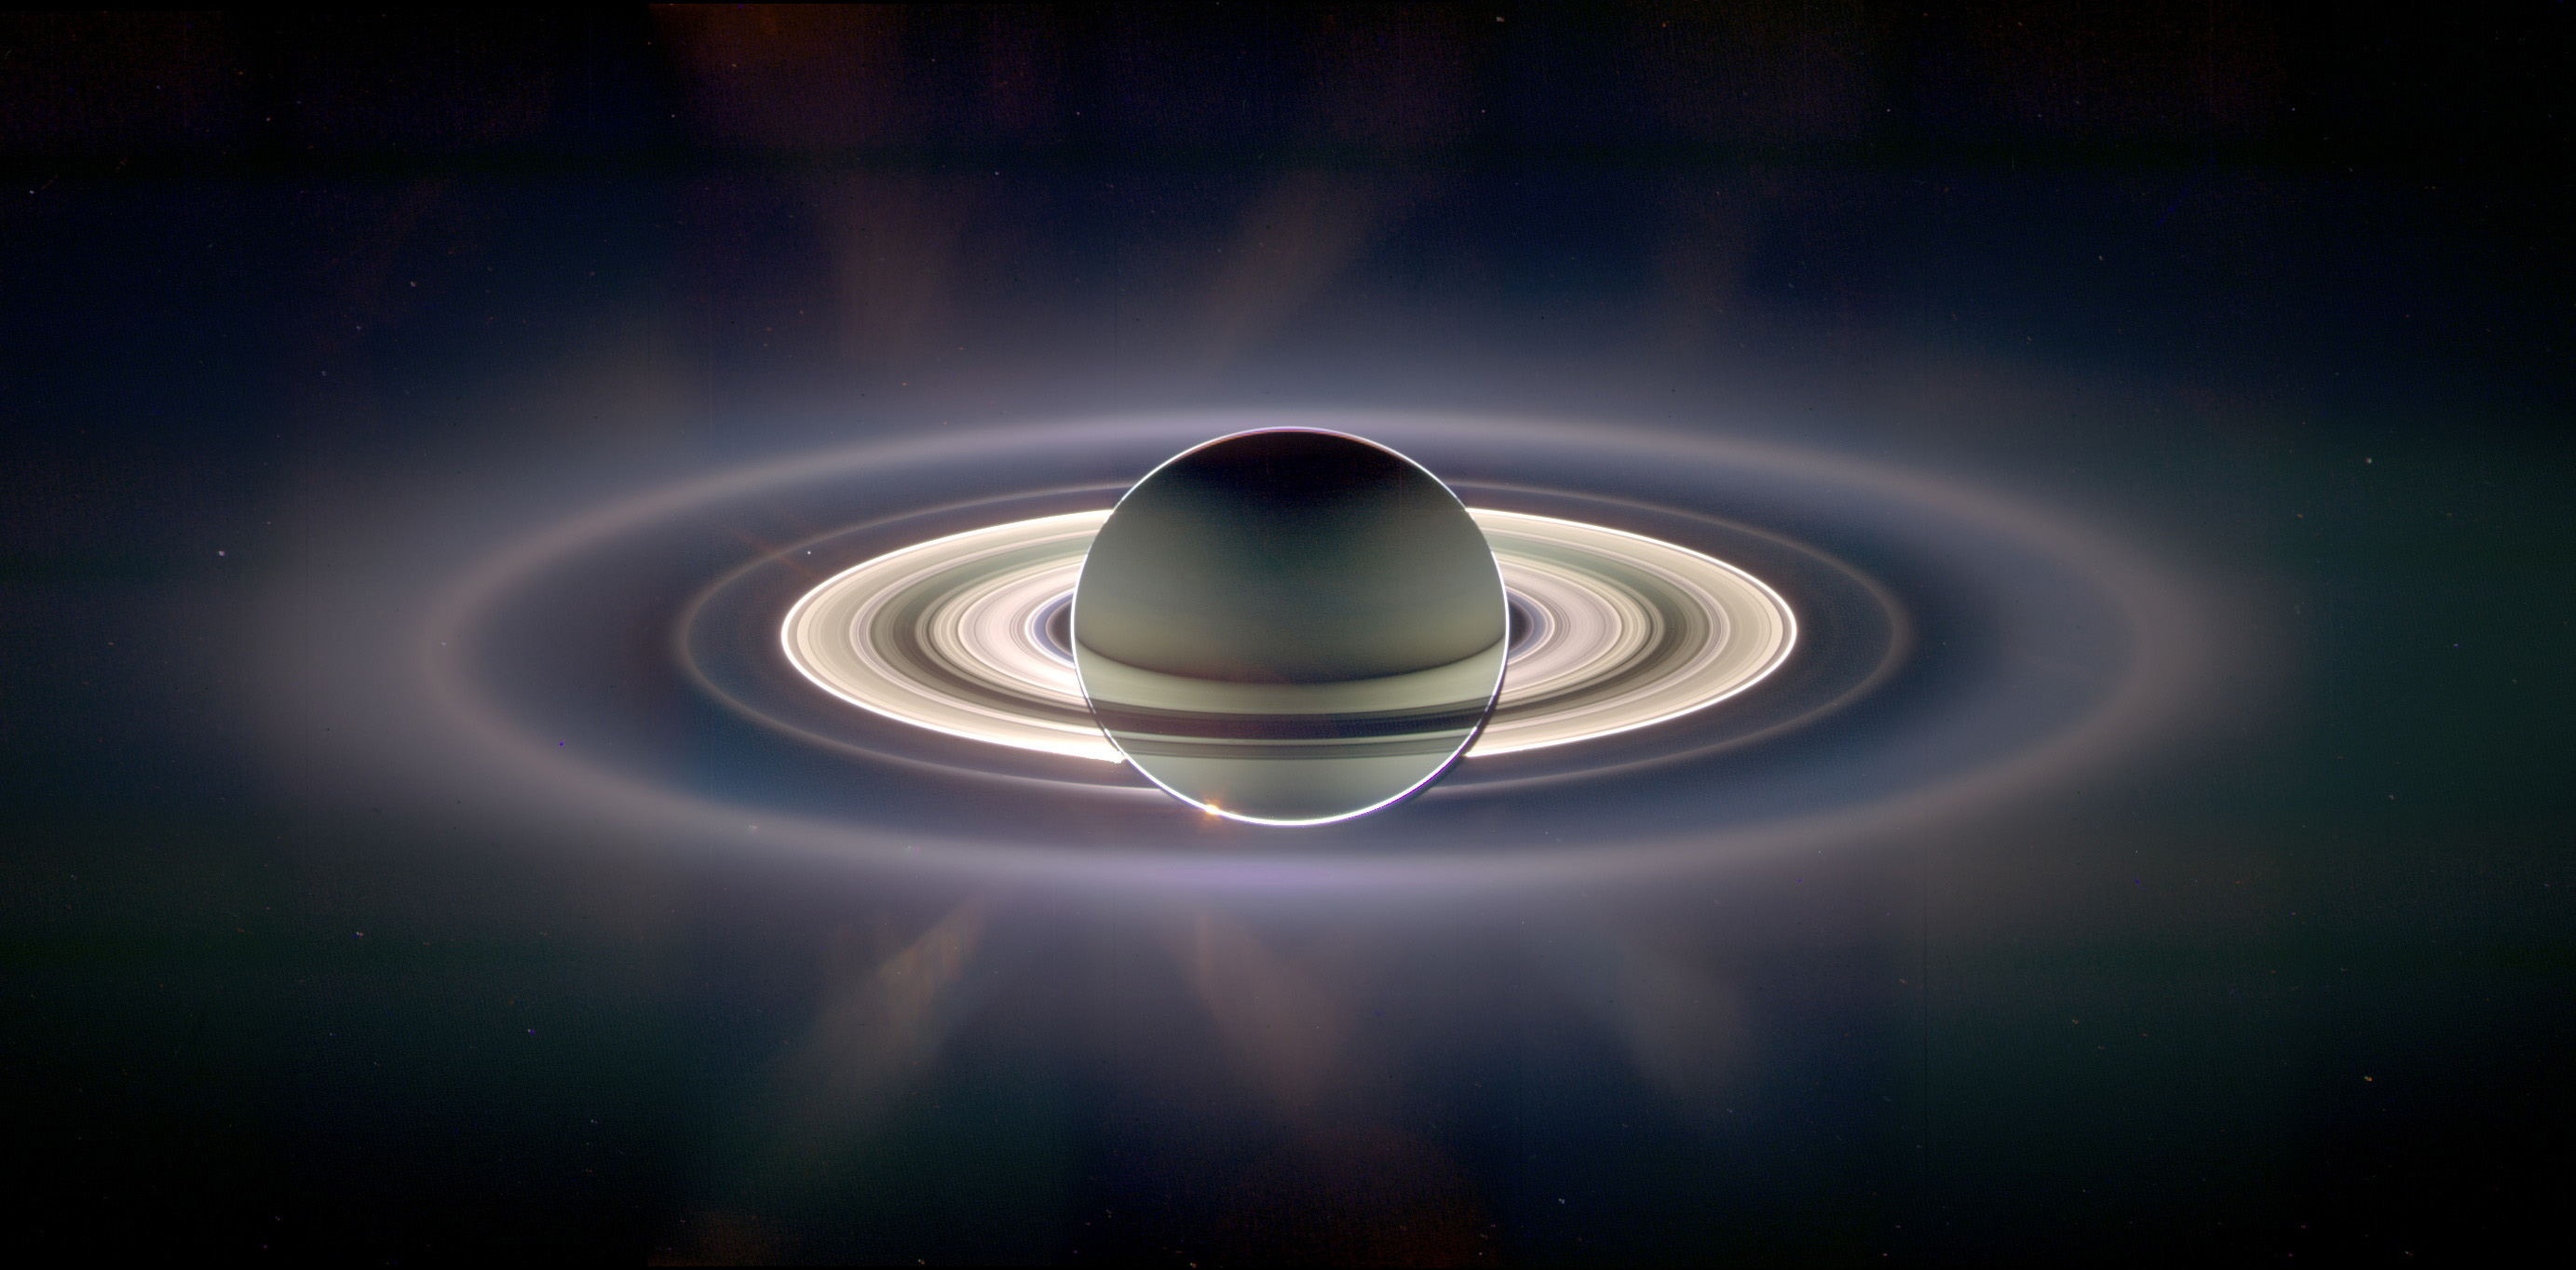
\includegraphics[width=\textwidth]{newrings_cassini_big.jpg}    
    \label{fig:saturn_rings}
  \end{figure}
  
\end{frame}

\begin{frame}[fragile]{Полидисперсность}
  Материал колец Сатурна в основном состоит из водяного льда, и варьируется в размерах
  от нескольких микрометров до нескольких десятков метров 

  \begin{figure}[h]
    \centering
    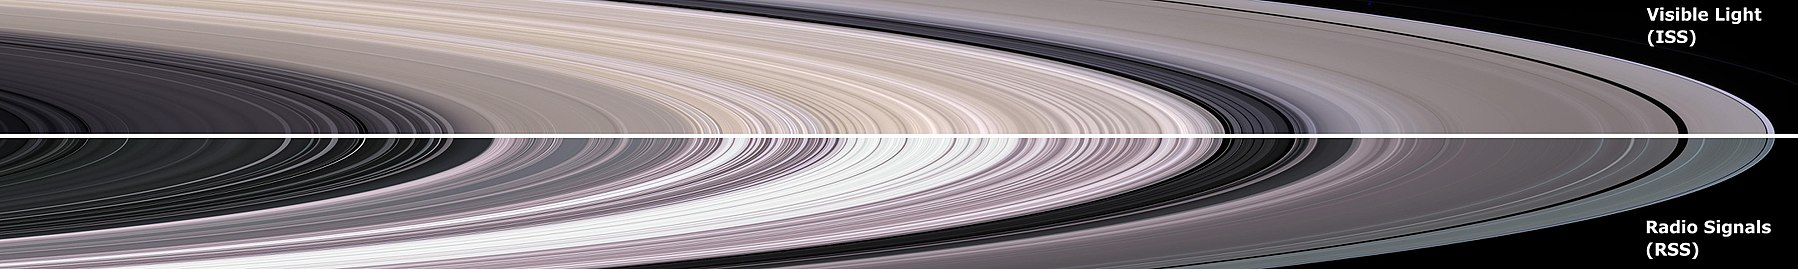
\includegraphics[width=\textwidth]{1800px-Saturn's_rings_in_visible_light_and_radio.jpg}    
    \label{fig:ring_structure_gas}
  \end{figure}
\end{frame}

\section{Кинетическое описание}

\begin{frame}{Функция распределения}
  
  Статистическая система описывается функцией распределения $f(t,m,\br,\bv)$ в фазовом пространстве $\br,\;\bv$
  и имеет следующее свойство

  \begin{equation}
    dN(t,m,\br,\bv)=f(t,m,\br,\bv)dv_xdv_ydv_z
  \end{equation}

  где $dN(t,m,\br,\bv)$ --- число частиц локализованных вокруг координаты $\br$ и имеющих скорости
  в диапазоне от $\bv$ до $\bv+d\bv$

\end{frame}

\begin{frame}[fragile]{Уравнение Больцмана}
	Эволюция функции распределения подчиняется уравнению Больцмана

  \begin{equation}
    \frac{\pd f}{\pd t}+\bv\frac{\pd f}{\pd\br}+\bw\frac{\pd f}{\pd\bv}=I_c(t,m,\br,\bv)\;,
  \end{equation}
  где $I_c(t,m,\br,\bv)$ --- интеграл столкновений
  
\end{frame}

\begin{frame}[fragile]{Механика столкновений}
  Скорости частиц после столкновения
  \begin{equation}
    \begin{split}
      \bv'_i&=\bv_i-\frac{\mu}{m_i}(1+\varepsilon)(\bg\cdot\bn)\bn\;,\\
      \bv'_j&=\bv_j+\frac{\mu}{m_j}(1+\varepsilon)(\bg\cdot\bn)\bn\;,
    \end{split}
  \end{equation}
  где $\mu=\cfrac{m_im_j}{m_i+m_j}$ --- эффективная масса столкновения
\end{frame}

\begin{frame}[fragile]{Механика столкновений}
  Изменение кинетической энергии при столкновении
  \begin{equation}
    \begin{split}
      \delta E_i&=-\mu(1+\varepsilon)(\bg\cdot\bn)(\bv_C\cdot\bn)-\frac{1-\varepsilon^2}{2}\frac{\mu^2}{m_i}(\bg\cdot\bn)^2\;,\\
      \delta E_j&=+\mu(1+\varepsilon)(\bg\cdot\bn)(\bv_C\cdot\bn)-\frac{1-\varepsilon^2}{2}\frac{\mu^2}{m_j}(\bg\cdot\bn)^2\;,
    \end{split}
  \end{equation}
  где $(m_i+m_j)\bv_C=m_i\bv_i+m_j\bv_j$ --- скорость центра масс
\end{frame}

\begin{frame}[fragile]{Нарушение равнораспределения энергии}
  Частицы с разными массами диссипируют разное количество энергии

  \begin{equation}
    \left(\frac{\delta E_i}{\delta E_j}\right)_{diss}=\frac{m_j}{m_i}
  \end{equation}
  чем \alert{меньше} масса частицы, тем \alert{больше} энергии она теряет. Полная потеря энергии
  \begin{equation}
    \delta E_i+\delta E_j=-\frac{1-\eps^2}{2}\mu(\bg\cdot\bn)^2
  \end{equation}

\end{frame}

\begin{frame}[fragile]{Интеграл столкновений}
  В общем виде интеграл столкновений для гранулярных газов имеет вид
  \begin{equation}
    \begin{split}
      &I_c(t,m_i,\br,\bv_i) = \int dm_j\eta(m_j)\sigma_{ij}\int d\bv_j\int d\bn\Theta(-\bg\cdot\bn)\vert\bg\cdot\bn\vert\times\\
      &\times\left(\frac{1}{\eps^2}f(t,m_i,\br,\bv''_i)f(t,m_j,\br,\bv''_j)-f(t,m_i,\br,\bv_i)f(t,m_j,\br,\bv_j)\right)
    \end{split}
  \end{equation}

  где $\bv^{''}_i$ и $\bv^{''}_j$ --- скорости обратных столкновений
\end{frame}

\section{Гидродинамическое описание}

\begin{frame}[fragile]{Условия применимости}
  Гидродинамическое приближение подразумевает описание системы только через его \alert{макроскопические} параметры.
  Для существования возможности такого описания необходимы условия
  \begin{equation}
    \sigma\ll\ell\ll L
  \end{equation}
\end{frame}

\begin{frame}[fragile]{Макроскопические переменные}
  Все макропараметры определяются как моменты вектора скорости частиц
  \begin{equation}
    \begin{split}
      \rho(t,m,\br) &= \int mf(t,m,\br,\br)d\bv\;,\\
      \rho\bu(t,m,\br) &= \int m\bv f(t,m,\br,\bv)d\bv\;,\\
      \frac{3}{2}nT(t,m,\br) &= \int \frac{m\bc^2}{2}f(t,m,\br,\bv)d\bv\;,
    \end{split}
  \end{equation}
  где $\bc=\bv-\bu(t,m,\br)$ --- локальная скорость частиц
\end{frame}

\begin{frame}[fragile]{Уравнения переноса}
  Интегрируя уравнение Больцмана по соответствующим моментам скоростей частиц получаем
  \begin{equation}
    \begin{split}
      &\frac{\pd\rho}{\pd t}+\frac{\pd}{\pd r_{\alpha}}(\rho u_{\alpha})=0\;,\\
      &\frac{\pd(\rho u_\alpha)}{\pd t} + \frac{\pd}{\pd r_\beta}(\rho u_\alpha u_\beta) = 
  -\frac{\pd\left(nT\right)}{\pd r_\alpha} - \frac{\pd\pi_{\ab}}{\pd r_\beta} + \rho w_\alpha\;,\\
  &\frac{\pd}{\pd t}\left(\frac{3}{2}nT+\frac{\rho\bu^2}{2}\right)+
  \frac{\pd}{\pd r_\alpha}u_\alpha\left(\frac{5}{2}nT+\frac{\rho\bu^2}{2}\right)+\\
  &+\frac{\pd}{\pd r_\alpha}(\pi_{\ab}u_\beta)
  +\frac{\pd q_\alpha}{\pd r_\alpha}=\rho\bw\cdot\bu-T\cdot\alert{\xi}\;.
    \end{split}
  \end{equation}

\end{frame}

\begin{frame}[fragile]{Охлаждения системы}
  Скорость охлаждения системы 
  \begin{equation}
  \begin{split}
    \xi(t,m_i,\br,T_i)&=-\frac{n_i}{T_i}\int d\chi_i \omega_{ij}(-A_{ij}T_i+B_{ij}(T_j-T_i))\;,\\
    A_{ij} &= \left(1-\eps^2\right)\frac{\mu}{m_i}\;,\\
    B_{ij} &= \left(1+\eps\right)^2\frac{\mu^2}{m_im_j}\;.
  \end{split}
  \end{equation}
  где $\omega_{ij}$ --- частота столкновений частиц. 

\end{frame}

\begin{frame}{Figures}
  \begin{figure}
    \newcounter{density}
    \setcounter{density}{20}
    \begin{tikzpicture}
      \def\couleur{alerted text.fg}
      \path[coordinate] (0,0)  coordinate(A)
                  ++( 90:5cm) coordinate(B)
                  ++(0:5cm) coordinate(C)
                  ++(-90:5cm) coordinate(D);
      \draw[fill=\couleur!\thedensity] (A) -- (B) -- (C) --(D) -- cycle;
      \foreach \x in {1,...,40}{%
          \pgfmathsetcounter{density}{\thedensity+20}
          \setcounter{density}{\thedensity}
          \path[coordinate] coordinate(X) at (A){};
          \path[coordinate] (A) -- (B) coordinate[pos=.10](A)
                              -- (C) coordinate[pos=.10](B)
                              -- (D) coordinate[pos=.10](C)
                              -- (X) coordinate[pos=.10](D);
          \draw[fill=\couleur!\thedensity] (A)--(B)--(C)-- (D) -- cycle;
      }
    \end{tikzpicture}
    \caption{Rotated square from
    \href{http://www.texample.net/tikz/examples/rotated-polygons/}{texample.net}.}
  \end{figure}
\end{frame}
\begin{frame}{Tables}
  \begin{table}
    \caption{Largest cities in the world (source: Wikipedia)}
    \begin{tabular}{lr}
      \toprule
      City & Population\\
      \midrule
      Mexico City & 20,116,842\\
      Shanghai & 19,210,000\\
      Peking & 15,796,450\\
      Istanbul & 14,160,467\\
      \bottomrule
    \end{tabular}
  \end{table}
\end{frame}
\begin{frame}{Blocks}
  Three different block environments are pre-defined and may be styled with an
  optional background color.

  \begin{columns}[T,onlytextwidth]
    \column{0.5\textwidth}
      \begin{block}{Default}
        Block content.
      \end{block}

      \begin{alertblock}{Alert}
        Block content.
      \end{alertblock}

      \begin{exampleblock}{Example}
        Block content.
      \end{exampleblock}

    \column{0.5\textwidth}

      \metroset{block=fill}

      \begin{block}{Default}
        Block content.
      \end{block}

      \begin{alertblock}{Alert}
        Block content.
      \end{alertblock}

      \begin{exampleblock}{Example}
        Block content.
      \end{exampleblock}

  \end{columns}
\end{frame}
\begin{frame}{Math}
  \begin{equation*}
    e = \lim_{n\to \infty} \left(1 + \frac{1}{n}\right)^n
  \end{equation*}
\end{frame}
\begin{frame}{Line plots}
  \begin{figure}
    \begin{tikzpicture}
      \begin{axis}[
        mlineplot,
        width=0.9\textwidth,
        height=6cm,
      ]

        \addplot {sin(deg(x))};
        \addplot+[samples=100] {sin(deg(2*x))};

      \end{axis}
    \end{tikzpicture}
  \end{figure}
\end{frame}
\begin{frame}{Bar charts}
  \begin{figure}
    \begin{tikzpicture}
      \begin{axis}[
        mbarplot,
        xlabel={Foo},
        ylabel={Bar},
        width=0.9\textwidth,
        height=6cm,
      ]

      \addplot plot coordinates {(1, 20) (2, 25) (3, 22.4) (4, 12.4)};
      \addplot plot coordinates {(1, 18) (2, 24) (3, 23.5) (4, 13.2)};
      \addplot plot coordinates {(1, 10) (2, 19) (3, 25) (4, 15.2)};

      \legend{lorem, ipsum, dolor}

      \end{axis}
    \end{tikzpicture}
  \end{figure}
\end{frame}
\begin{frame}{Quotes}
  \begin{quote}
    Veni, Vidi, Vici
  \end{quote}
\end{frame}

{%
\setbeamertemplate{frame footer}{My custom footer}
\begin{frame}[fragile]{Frame footer}
    \themename defines a custom beamer template to add a text to the footer. It can be set via
    \begin{verbatim}\setbeamertemplate{frame footer}{My custom footer}\end{verbatim}
\end{frame}
}

\begin{frame}{References}
  Some references to showcase [allowframebreaks] \cite{knuth92,ConcreteMath,Simpson,Er01,greenwade93}
\end{frame}

\section{Conclusion}

\begin{frame}{Summary}

  Get the source of this theme and the demo presentation from

  \begin{center}\url{github.com/matze/mtheme}\end{center}

  The theme \emph{itself} is licensed under a
  \href{http://creativecommons.org/licenses/by-sa/4.0/}{Creative Commons
  Attribution-ShareAlike 4.0 International License}.

  \begin{center}\ccbysa\end{center}

\end{frame}

{\setbeamercolor{palette primary}{fg=black, bg=yellow}
\begin{frame}[standout]
  Questions?
\end{frame}
}

\appendix

\begin{frame}[fragile]{Backup slides}
  Sometimes, it is useful to add slides at the end of your presentation to
  refer to during audience questions.

  The best way to do this is to include the \verb|appendixnumberbeamer|
  package in your preamble and call \verb|\appendix| before your backup slides.

  \themename will automatically turn off slide numbering and progress bars for
  slides in the appendix.
\end{frame}

\begin{frame}[allowframebreaks]{References}

  \bibliography{demo}
  \bibliographystyle{abbrv}

\end{frame}

\end{document}
